% SC4040 --- Chapter 2: Randomization (0->100 ground-up)
\chapter{Randomized Algorithms}
\label{ch:random}

\begin{quote}
\emph{``Randomness is not chaos --- it is a resource.''} By letting the algorithm flip coins, we obtain simplicity, speed, and robustness that deterministic algorithms struggle to match. We build the probabilistic toolkit from scratch.
\end{quote}

\noindent\fbox{\parbox{\dimexpr\linewidth-2\fboxsep-2\fboxrule}{%
\textbf{From zero: probability from coin flips up.} We define sample spaces, expectation, and concentration before any algorithm. No prior randomised-algorithms course assumed; every tail bound is derived when needed.}}
\vspace{0.4em}

\section*{Learning Outcomes}
After this chapter you will be able to:
\begin{enumerate}[label=(L\arabic*)]
    \item analyse expected running time of randomised QuickSort via indicator variables;
    \item prove correctness and success probability of Karger's min-cut algorithm;
    \item analyse universal hashing and its expected $O(1)$ dictionary operations;
    \item prove correctness and error bounds for the Miller--Rabin primality test;
    \item apply linearity of expectation, Markov, and Chernoff reasoning.
\end{enumerate}

% ============================================================
\section{Probability Toolkit in One Page}
\label{sec:prob-toolkit}

A \emph{sample space} $\Omega$ lists outcomes; event $A\subseteq\Omega$ has $\Pr[A]=|A|/|\Omega|$ (uniform) or $\sum_{\omega\in A}p(\omega)$ generally. Random variable $X:\Omega\to\mathbb{R}$; expectation $\mathbb{E}[X]=\sum_{\omega}X(\omega)p(\omega)$. Key tools:
\begin{itemize}
    \item \textbf{Linearity:} $\mathbb{E}[X+Y]=\mathbb{E}[X]+\mathbb{E}[Y]$ even when $X,Y$ dependent.
    \item \textbf{Indicator:} $I_A=1$ if $A$ occurs else $0$; $\mathbb{E}[I_A]=\Pr[A]$.
    \item \textbf{Markov:} $\Pr[X\ge t]\le\mathbb{E}[X]/t$ for $X\ge0$.
    \item \textbf{Union bound:} $\Pr[\bigcup_i A_i]\le\sum_i\Pr[A_i]$.
\end{itemize}

\begin{figure}[h]\centering
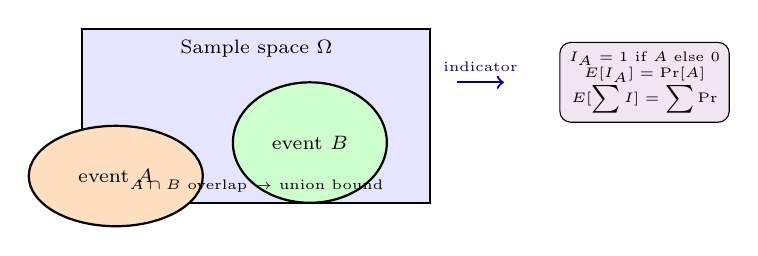
\begin{tikzpicture}[scale=0.85,font=\scriptsize]
\draw[thick,fill=blue!10] (0,0) rectangle (5.2,2.6);
\node at (2.6,2.3) {Sample space $\Omega$};
\draw[thick,fill=orange!25] (0.5,0.4) ellipse (1.3 and 0.75) node {event $A$};
\draw[thick,fill=green!20] (3.4,0.9) ellipse (1.15 and 0.9) node {event $B$};
\node[font=\tiny] at (2.6,0.25) {$A\cap B$ overlap $\to$ union bound};
\draw[->,thick,blue!60!black] (5.6,1.8)--(6.3,1.8) node[midway,above,font=\tiny] {indicator};
\node[draw,rounded corners,fill=violet!10,align=center,font=\tiny] at (8.4,1.8) {$I_A=1$ if $A$ else $0$\\$\mathbb{E}[I_A]=\Pr[A]$\\$\mathbb{E}[\sum I]=\sum\Pr$};
\end{tikzpicture}
\caption{Events as regions; indicator variables turn counting into expectation via linearity --- the workhorse of randomised analysis.}
\label{fig:prob-toolkit}
\end{figure}

% ============================================================
\section{Randomised QuickSort: No Adversary Can Hurt You}
\label{sec:rqs}

Deterministic QuickSort has $\Theta(n^2)$ worst case (sorted input + first-element pivot). Randomising the pivot removes any bad \emph{input}: expected time is $O(n\log n)$ for \emph{every} input, over the coin flips.

Idea: elements $z_1<\cdots<z_n$ sorted. Let $X_{ij}=1$ if $z_i$ and $z_j$ are ever compared. Comparison happens iff among $Z_{ij}=\{z_i,\dots,z_j\}$, either $z_i$ or $z_j$ is chosen as pivot first --- prob.\ $2/(j-i+1)$.

\begin{lstlisting}[language=Python]
import random
def quicksort(arr):
    """Randomized QuickSort -- expected O(n log n)."""
    if len(arr) <= 1:
        return arr
    pivot = random.choice(arr)          # random pivot
    left  = [x for x in arr if x < pivot]
    mid   = [x for x in arr if x == pivot]
    right = [x for x in arr if x > pivot]
    return quicksort(left) + mid + quicksort(right)

def expected_comparisons(n):
    # E[comparisons] = sum_{i<j} 2/(j-i+1) = O(n log n)
    return sum(2.0/(j-i+1) for i in range(n) for j in range(i+1, n))
\end{lstlisting}

\begin{theorem}[Randomised QuickSort]
$\mathbb{E}[\text{comparisons}]=\sum_{i<j}\tfrac{2}{j-i+1}=O(n\log n)$. Hence expected time $O(n\log n)$ and $\Pr[T\ge c\,n\log n]$ is small by Markov.
\end{theorem}
\begin{proof}
$\mathbb{E}[\sum_{i<j}X_{ij}]=\sum_{i<j}\Pr[X_{ij}=1]=\sum_{i<j}2/(j-i+1)$. Group by $k=j-i+1$: inner sum is $(n-k+1)\cdot2/k$, so total $\le2n\sum_{k=2}^{n}1/k=2nH_n=O(n\log n)$.
\end{proof}

% ============================================================
\section{Karger's Min-Cut: Flip, Contract, Succeed}
\label{sec:karger}

\textsc{Global Min-Cut}: smallest edge set whose removal disconnects $G$. Karger's idea --- randomly contract edges until $2$ supernodes remain; the edges between them are a cut.

\begin{figure}[h]\centering
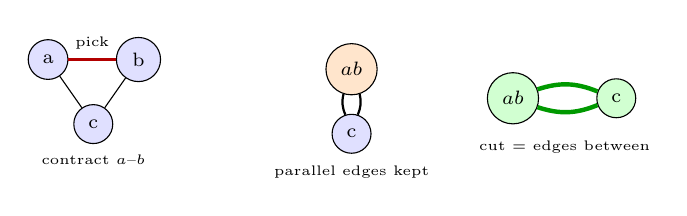
\begin{tikzpicture}[scale=0.82,font=\scriptsize]
\begin{scope}
\node[circle,draw,fill=blue!12,minimum size=14pt] (a) at (0,1) {a};
\node[circle,draw,fill=blue!12,minimum size=14pt] (b) at (1.4,1) {b};
\node[circle,draw,fill=blue!12,minimum size=14pt] (c) at (0.7,0) {c};
\draw[thick] (a)--(b) node[midway,above,font=\tiny] {pick}; \draw (b)--(c); \draw (a)--(c);
\draw[thick,red!70!black] (a)--(b);
\node[font=\tiny] at (0.7,-0.55) {contract $a$--$b$};
\end{scope}
\begin{scope}[xshift=4cm]
\node[circle,draw,fill=orange!20,minimum size=18pt] (ab) at (0.7,0.85) {$ab$};
\node[circle,draw,fill=blue!12,minimum size=14pt] (c2) at (0.7,-0.15) {c};
\draw[thick] (ab) to[bend left=18] (c2); \draw[thick] (ab) to[bend right=18] (c2);
\node[font=\tiny] at (0.7,-0.75) {parallel edges kept};
\end{scope}
\begin{scope}[xshift=7.2cm]
\node[circle,draw,fill=green!18,minimum size=14pt] (x) at (0,0.4) {$ab$};
\node[circle,draw,fill=green!18,minimum size=14pt] (y) at (1.6,0.4) {c};
\draw[ultra thick,green!60!black] (x) to[bend left=20] (y); \draw[ultra thick,green!60!black] (x) to[bend right=20] (y);
\node[font=\tiny] at (0.8,-0.35) {cut = edges between};
\end{scope}
\end{tikzpicture}
\caption{Karger contraction: pick a random edge, merge endpoints (parallel edges preserved). After $n-2$ contractions, the remaining edges form a cut; a fixed min-cut survives with prob.\ $2/n(n-1)$.}
\label{fig:karger}
\end{figure}

Fix a min-cut $C$ of size $k$. An edge of $C$ is contracted only if we pick one of its $k$ edges among $\ge nk/2$ total (since min degree $\ge k$). So survival prob.\ per step $i$ (with $r=n-i+1$ supernodes) is $\ge1-2/r$. Multiplying:
\[
\Pr[\text{$C$ survives}] \ge \prod_{r=3}^{n}\!\left(1-\tfrac{2}{r}\right)=\tfrac{2}{n(n-1)}.
\]
Repeating $O(n^2\log n)$ times and taking the smallest cut boosts success to $1-1/n$. Karger--Stein improves to $O(n^2\log^3 n)$ via recursion.

\begin{lstlisting}[language=Python]
import random
def karger_once(n, edges):
    """One trial of Karger. edges: list of (u,v). Returns cut size."""
    parent = list(range(n))
    def find(x):
        while parent[x]!=x: parent[x]=parent[parent[x]]; x=parent[x]
        return x
    verts = n
    while verts > 2:
        u,v = random.choice(edges)
        ru, rv = find(u), find(v)
        if ru == rv: continue
        parent[rv] = ru; verts -= 1
    # count edges crossing the two supernodes
    cut = sum(1 for u,v in edges if find(u) != find(v))
    return cut
\end{lstlisting}

% ============================================================
\section{Universal Hashing: Randomness Tames Adversaries}
\label{sec:hashing}

A hash family $\mathcal{H}=\{h:U\to[m]\}$ is \emph{universal} if for $x\neq y$, $\Pr_{h\sim\mathcal{H}}[h(x)=h(y)]\le1/m$. Construction over prime $p\ge|U|$: $h_{a,b}(x)=((ax+b)\bmod p)\bmod m$ with $a\neq0$ random.

With chaining, expected chain length for $n$ keys is $n/m$; with $m=\Theta(n)$, expected $O(1)$ per operation regardless of input distribution --- the random choice of $h$ defeats any fixed bad set.

% ============================================================
\section{Miller--Rabin: Testing Primality by Witnesses}
\label{sec:miller-rabin}

Write $n-1=2^s d$ ($d$ odd). For base $a$, check $a^d\equiv1$ or $a^{2^rd}\equiv-1$ for some $r<s$. Composite $n$ has $\ge3/4$ of bases as witnesses (Rabin). Repeating $t$ independent bases: error $\le4^{-t}$.

\begin{lstlisting}[language=Python]
import random
def is_probable_prime(n, t=10):
    """Miller-Rabin. Returns False=certainly composite, True=probably prime."""
    if n < 2: return False
    if n % 2 == 0: return n == 2
    d, s = n-1, 0
    while d % 2 == 0: d //= 2; s += 1
    for _ in range(t):
        a = random.randrange(2, n-1)
        x = pow(a, d, n)
        if x == 1 or x == n-1: continue
        for _ in range(s-1):
            x = pow(x, 2, n)
            if x == n-1: break
        else:
            return False  # witness: definitely composite
    return True  # probably prime, error <= 4^{-t}
\end{lstlisting}

\begin{figure}[h]\centering
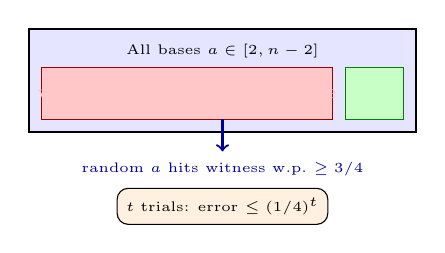
\begin{tikzpicture}[scale=0.82,font=\scriptsize]
\draw[thick,fill=blue!10] (0,0) rectangle (6,1.6);
\node[font=\tiny,align=center] at (3,1.25) {All bases $a\in[2,n-2]$};
\fill[red!22,draw=red!60!black] (0.2,0.2) rectangle (4.7,1.0) node[midway] {witnesses $\ge 3/4$ if $n$ composite};
\fill[green!22,draw=green!50!black] (4.9,0.2) rectangle (5.8,1.0) node[midway,font=\tiny] {liars};
\draw[->,thick,blue!60!black] (3,0.2)--(3,-0.3) node[below,font=\tiny] {random $a$ hits witness w.p.\ $\ge3/4$};
\node[draw,rounded corners,fill=orange!12,font=\tiny,align=center] at (3,-1.15) {$t$ trials: error $\le(1/4)^t$};
\end{tikzpicture}
\caption{Miller--Rabin: if $n$ is composite, at least $3/4$ of bases expose it. Repeating shrinks error exponentially.}
\label{fig:miller-rabin}
\end{figure}

% ============================================================
\section{Worked Example: Balls into Bins}
\label{sec:balls-bins}

Throw $n$ balls into $n$ bins uniformly. Expected load $1$ per bin, but max load is $\Theta(\log n/\log\log n)$ w.h.p.\ via Chernoff + union bound: $\Pr[\text{bin }i\ge k]\le\binom{n}{k}(1/n)^k\le(e/k)^k$. Setting $k=3\log n/\log\log n$ makes this $o(1/n)$; union over $n$ bins gives w.h.p.\ bound. This underpins hashing and load balancing analyses.

% ============================================================
\section{Concentration: Chernoff and Beyond}
\label{sec:chernoff}

Markov is weak. For independent $X_i\in[0,1]$ with $X=\sum X_i$ and $\mu=\mathbb{E}[X]$, Chernoff gives $\Pr[X\ge(1+\delta)\mu]\le\exp(-\mu\delta^2/3)$ for $\delta\in[0,1]$, and Hoeffding handles bounded variables without identical distribution. These power the analysis of balls-into-bins ($O(\log n/\log\log n)$ max load), random sampling, and Miller--Rabin amplification. The trick: bound moment-generating functions $\mathbb{E}[e^{tX}]$ then optimise $t$.

% ============================================================
\section{Chapter Notes}
Motwani--Raghavan is the classic randomised-algorithms text. Karger (1993) and Karger--Stein (1996) remain the simplest min-cut algorithms. Miller--Rabin is used in every cryptographic library; deterministic polynomial-time primality is AKS (2004) but slower in practice.

% ============================================================
\section{Exercises}
\label{sec:ch02-exercises}
\begin{enumerate}[label=E2.\arabic*, leftmargin=*, itemsep=0.7em]
    \item \textbf{QuickSort tail bound.} Use Markov's inequality to bound $\Pr[T\ge 10\,\mathbb{E}[T]]$ for randomised QuickSort. Can you get a stronger bound using the fact that $\Pr[X_{ij}]$ events are not independent? Discuss.
    \item \textbf{Karger amplification.} Show that running Karger $c\,n^2\ln n$ times and taking the minimum cut yields success probability $\ge1-n^{-c'}$ for suitable $c'$. Compute $c'$ as a function of $c$.
    \item \textbf{Universal hashing construction.} Prove that $h_{a,b}(x)=((ax+b)\bmod p)\bmod m$ with prime $p\ge|U|$ and uniform $a\in[1,p-1],b\in[0,p-1]$ is universal. Count collisions for $x\neq y$.
    \item \textbf{Miller--Rabin error.} Prove that repeating Miller--Rabin $t$ times gives error at most $4^{-t}$ even when the $t$ bases are chosen independently. Why does the $3/4$ witness fraction imply this?
    \item \textbf{Hash table expectation.} With $n$ keys hashed into $m=n$ buckets via a universal family and chaining, prove expected maximum chain length is $O(\log n/\log\log n)$ is not needed --- simply show expected lookup cost is $O(1)$ and expected number of colliding pairs is $\le n/2$.
\end{enumerate}
% End of Chapter 2
